\documentclass[xetex,aspectratio=43]{beamer}

\usepackage{res/lections}

\preamble

\title[АП и ВП]{Адресное пространство,\\физическая и виртуальная память}

\begin{document}

    \titleslide

    \tocslide

\begin{frame}{Основные термины}
    \begin{itemize}
        \item
        \defn{Физический адрес}{номер байта в оперативной памяти,
        начиная с нулевого}
        \item
        \defn{Виртуальный (Логический) адрес}{адрес, с
        которым работает прикладное ПО, например, значение указателя}
        \item
        \defn{Адресное пространство}{множество логических адресов}
        \item
        \defn{Адресное преобразование}{вычисление физического адреса по
        виртуальному}
    \end{itemize}

\end{frame}

\section{Виды адресации (кроме страничной)}

\subsection{Прямая адресация}

\begin{frame}{Сущность прямой адресации}
    \begin{itemize}
        \item
        \defn{Прямая адресация}{способ адресации, при которой физический
        адрес равен логическому}
    \end{itemize}

    Т.е. адресное преобразование тривиально, фактически «указатель» сразу
    выдаётся на шину адреса
\end{frame}

\begin{frame}{Свойства прямой адресации}
    \begin{itemize}
        \item
        Типично для восьмибитной шины данных --- 16-битные внутренняя арифметика и шина адреса
        \item
        Изначально даже возможные 64KiB не использовались. Примеры:

        \begin{itemize}
            \item Sinclair ZX 80 --- ЦП Z80 (64K), но только 1К ОЗУ; Sinclair ZX
            \item Spectrum --- тоже Z80, но от 16 К ОЗУ
        \end{itemize}
    \end{itemize}

    \pause

    Для офисных приложений и игр нужны графика и больше памяти
\end{frame}

\subsection{Банковые расширения}

\begin{frame}{Сущность банковых расширений}
        \begin{figure}
            \includegraphics[page=2, width=0.75\textwidth]{img/06.Mem_Models-crop.pdf}
        \end{figure}

        \defn{Банковая адресация}{способ адресации, при которой адресное
        пространство разделяется на \emph{банки адресного пространства}, которым
        в соответствие ставятся \emph{банки оперативной памяти}}

        Соответствие обычно не произвольное, варианты ограничены
\end{frame}

\begin{frame}{Свойства банковых расширений}
        Хорошо

        \begin{itemize}
            \tightlist
            \item
            Процессор тот же, вообще вмешательство в архитектуру минимально
            \item
            Дешево стоит
            \item
            Память можно расширять произвольно, доступно радиолюбителям
            \item
            Сравнительно удобно работать с данными
        \end{itemize}

        Плохо

        \begin{itemize}
            \tightlist
            \item
            Работает не быстро
            \item
            Программируется через порты; тяжело менять банки кода, особенно для:

            \begin{itemize}
                \tightlist
                \item
                Вызова процедур
                \item
                Прерываний
                \item
                Переключения задач
            \end{itemize}
            \item
            Разные расширения часто несовместимы
        \end{itemize}
\end{frame}

\begin{frame}[fragile]{Пример 1: ZX Spectrum 128K}
    \href{http://www.worldofspectrum.org/faq/reference/128kreference.htm}{ZX
        Spectrum 128K}

    { \scriptsize \begin{verbatim}
        0xFFFF --+--------+--------+--------+--------+--------+--------+--------+
        | Bank 0 | Bank 1 | Bank 2 | Bank 3 | Bank 4 | Bank 5 | Bank 6 | Bank 7 |
        |        |        |(also at|        |        |(also at|        |        |
        |        |        | 0x8000)|        |        | 0x4000)|        |        |
        |        |        |        |        |        | screen |        | screen |
        + 0xC000 +--------+--------+--------+--------+--------+--------+--------+
        | Bank 2 |        Any one of these pages may be switched in.
        |        |
        |        |
        |        |
        + 0x8000 +---
        | Bank 5 |
        |        |
        |        |
        | screen |
        + 0x4000 +--------+
        | ROM 0  | ROM 1  | Either ROM may be switched in.
        |        |        |
        |        |        |
        |        |        |
        + 0x0000 +--------+
    \end{verbatim} }
\end{frame}

\begin{frame}{Пример 1: Как это реализовано}
    Адресное преобразование вычисляет номер банка ОЗУ по номеру банка
    (старшим 2 битам) АП. Отображение хранится в регистрах схемы MMU

    \begin{figure}
        \includegraphics[page=3,height=0.6\textheight]{img/06.Mem_Models-crop.pdf}
    \end{figure}

    Адресное преобразование:
    \(A_{ph} = \mathit{MMU}[A_{log\\; 14\ldots 15}] + A_{log\\; 0\dots 13}\)
\end{frame}

\begin{frame}{Пример 2: Окна в адресном пространстве IBM PC}
    Можно рассматривать, как вариант банковой системы

    \begin{figure}
        \includegraphics[page=4,height=0.4\textheight]{img/06.Mem_Models-crop.pdf}
    \end{figure}

    \begin{itemize}
        \tightlist
        \item
        Некоторые внешние устройства, например графические адаптеры,
        поддерживают до сих пор
        \item
        Использовалась в EMS --- сначала плата расширения, затем встроенная
        поддержка на материнской плате, затем эмуляция при помощи страничной
        адресации
    \end{itemize}

    \pause

    \begin{itemize}
        \tightlist
        \item
        Использовалась в XMS --- сразу чисто программное решение (эмуляция),
        Intel 80286+
    \end{itemize}

    Адресное преобразование: устройства перехватывают обращение к ОЗУ на
    системной шине
\end{frame}

\subsection{Совместимые расширения и эволюция ЦП}

\begin{frame}[fragile]{Расширение адресных регистров}
    Расширение адресных регистров

    \begin{itemize}
        \tightlist
        \item
        Старый машинный код не знает, что у адресного регистра есть старшая
        половинка
        \item
        Все переходы и обращения к данным в старом коде «короткие»
        \item
        Т.к. старые приложения не используют всю память, появляется внутренняя
        фрагментация
    \end{itemize}

    \pause

    Пример:

    \begin{itemize}
        \tightlist
        \item
        i8086 -- i80286 --- 16-битный регистр \texttt{BP}
        \item
        i80386 -- i80586 --- 32-битный регистр \texttt{EBP} (но младшие 16 бит
        доступны, как \texttt{BP})
        \item
        x86\_64 --- 64-битный регистр \texttt{RBP} (но доступны \texttt{EBP} и
        \texttt{BP})
    \end{itemize}

\end{frame}

\subsection{Сегментная адресация}

\begin{frame}{Смысл сегментной адресации}
    \begin{itemize}
        \item
        Компилятор (точнее, компоновщик) генерирует программу, в бинарном
        файле которой обозначены данные разных видов --- машинный код,
        статические данные (проинициализированные глобальные переменные) и
        т.д.
        \item
        Операционная система может размещать эти данные в физической памяти по
        своему усмотрению
        \item
        Получается, что нужен уровень косвенности, как при вызове API ядра
        через прерывания или спец. инструкции, только уже внутри программы.
    \end{itemize}
\end{frame}

\begin{frame}[fragile]{Реализация сегментной адресации (1): Жёсткие сегменты x86}
    В 16-битном режиме x86 полный указатель состоит из \emph{смещения}
    (адресный регистр) и \emph{номера сегмента} (хранится в сегментном
    регистре). Пример для x86 (i8086):

    \begin{itemize}
        \tightlist
        \item
        Адрес исполняемой инструкции \texttt{CS:IP} --- Code Segment,
        Instruction Pointer
        \item
        Адрес вершины стека \texttt{SS:SP} --- Stack Segment, Stack Pointer
        \item
        Адреса данных:

        \begin{itemize}
            \tightlist
            \item
            \texttt{DS:SI}, \texttt{ES:SI}, \texttt{DS:BX} и т.д., много
            сочетаний
        \end{itemize}
    \end{itemize}

    В ранних x86 защиты не было, и программа могла работать с разными
    сегментами * Обычно ОС (чаще всего DOS) выдавала ей по одному сегменту
    кода, стека и данных * Если 64К для чего-то из этого было мало, можно
    было использовать другие модели памяти, работая с разными сегментами.
    \href{http://www.c-jump.com/CIS77/ASM/Directives/D77_0030_models.htm}{Подробнее
        здесь}

    Адресное преобразование: \(A_{ph} = S \cdot 16 + O\)
\end{frame}

\begin{frame}{Реализация: Управляемые сегменты}

    \begin{figure}
        \includegraphics[page=3,height=0.55\textheight]{img/06.cache-and-vm-crop.pdf}
        \vspace{-5mm}
    \end{figure}

    \begin{itemize}
        \tightlist
        \item
        Произвольного размера
        \item
        Требуют специальных таблиц размещения (таблицы дескрипторов)
        \item
        Могут ассоциироваться с правами на хранение данных и кода и выполнение
        кода
    \end{itemize}

    \pause

    Если включена защита, процесс не может обращаться к чужим сегментам (как
    минимум должна «попросить разрешения» у ОС)

    Адресное преобразование: \(A_{ph} = T_{desc}[S] + O\)

\end{frame}

\section{Виртуальная память и страничная адресация}

\subsection{Реализация}

\begin{frame}{Что такое виртуальная память}
    \defn{Виртуальная память}{механизм работы с адресным
    пространством, превосходящим по размеру оперативную память или тот её
    фрагмент, который выделен данному процессу}

    ~

    Виртуальная память может по размеру превосходить физическую, и состоять
    из различных фрагментов, находящихся ОЗУ (по разным физическим адресам)
    или даже жесткого диска (за счёт чего и можно наращивать её размер). При
    этом адресное преобразование скрывает всю эту неоднородность от
    программы
\end{frame}

\begin{frame}{Предпосылки}
    \begin{block}{Задачи}
        \begin{itemize}
            \tightlist
            \item
            Ранние ЭВМ --- научные расчёты, обычно сравнительно небольшой код и
            объёмные данные. Данные можно обрабатывать порциями. ПО относительно
            недорого в масштабах системы
            \item
            Позже --- большее количество программ, больший объём кода. Большая
            относительная стоимость ПО
        \end{itemize}
    \end{block}

    \begin{block}{Решения}
        \begin{itemize}
            \tightlist
            \item
            Типичный способ работать с большим машинным кодом --- загружать его
            кусками --- \emph{оверлеями} (overlay). Иногда использовался и для DOS
            на PC.
            \item
            В некоторых архитектурах часть адресного пространства проецировалась
            на диск (или барабан), чтобы облегчить программисту работы
            \item
            \ldots{}
            \item
            Сделать прозрачную для программиста систему
        \end{itemize}
    \end{block}
\end{frame}

\begin{frame}{Страничная адресация: сущность}
    J. Fotheringham. Dynamic Storage Allocation in the Atlas Computer
    Including an Automatic Use of a Backing Store», Commun. of the ACM,
    vol.~4, pp.~435--436, 1961.

    Идея: разделить адресное пространство и ОЗУ на одинаковые по размеру страницы адресного
    пространства и страницы ОЗУ.

    \begin{figure}
        \includegraphics[page=3,height=0.55\textheight]{img/06.cache-and-vm-crop.pdf}
    \end{figure}
\end{frame}

\begin{frame}{Страничная адресация: реализация}
    \begin{figure}
        \includegraphics[page=5,height=0.55\textheight]{img/06.Mem_Models-crop.pdf}
    \end{figure}

    Адресное преобразование считывает таблицу страниц из ОЗУ и по номеру
    страницы АП находит номер страницы ОЗУ

    Адресное преобразование (пример 80386):
    \(A_{ph} = T_{pages}[A_{log\\; 12\ldots 31}] + A_{log\\; 0\ldots 11}\)
\end{frame}



\begin{frame}{Страничная адресация: свойства}
    \begin{itemize}
        \item
        Страницы небольшие и не пересекаются
        \item
        В отличие от жестких сегментов, часто могут <<гулять>> по физическим
        адресам под управлением ОС.
        \item
        Для управляемых страниц нужны таблицы размещения в основной памяти, к
        которым обращается ЦП \(\Rightarrow\) нужен хороший (и
        специально оптимизированный кэш)
        \item
        Удобны для реализации виртуальной памяти --- их можно выгружать и
        загружать без ведома пользовательского процесса
    \end{itemize}
\end{frame}

\begin{frame}{Виртуальная память на основе страничной адресации}
    \begin{itemize}
        \tightlist
        \item
        Изначально страницы процесса не проинициализированы
        \item
        По мере фактического обращения к памяти, страницам адресного
        пространства сопоставляются страницы памяти
        \item
        При нехватке памяти часть страниц процесса выгружаются на диск и
        помечаются, как выгруженные, освобождая физическую память для текущего
        и других процессов. Это называется \emph{вытеснением}
        \item На освободившееся место проецируются данные новой виртуальной страницы или
        страницы, подгруженной из подкачки.  Это называется \emph{замещением}
    \end{itemize}

    Термины \emph{вытеснение} и \emph{замещение} обычно отождествляют, т.к. первое нужно для второго, и второе за первым обычно следует

    \pause

    А что происходит, когда процесс обращается к не проинициализированной
    или выгруженной странице?

    \pause

    Процессор сам генерирует прерывание, обрабатывает которое драйвер
    виртуальной памяти
\end{frame}


\subsection{Вытеснение и замещение}

\begin{frame}{Стратегии вытеснения}
    \begin{itemize}
        \item
        Принцип Белади (L\'aszl\'o B\'el\'ady) --- вытеснить страницу, которая дольше
        всего не понадобится

        \pause

        \item
        Поскольку предсказать этого нельзя, используются различные стратегии.
        Самая популярная --- LRU (Least Recently Used) --- вытеснить страницу,
        к которой дольше всего не обращались
    \end{itemize}
\end{frame}

\begin{frame}{А что ещё вытесняется и замещается}

        \begin{figure}
            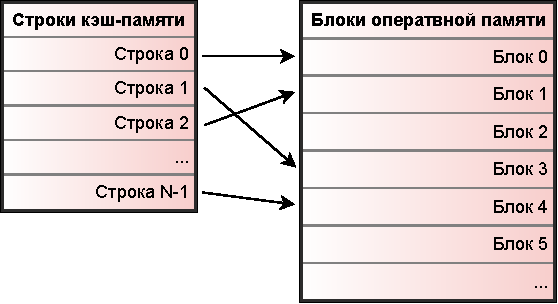
\includegraphics[page=1,height=0.45\textheight]{img/06.cache-and-vm-crop.pdf}
        \end{figure}

        \defn{Кэш-память}{специальный вид памяти между процессором и
        оперативной памятью, в которой хранятся копии используемых в данный
        момент фрагментов оперативной памяти}

        Кэш-память делится на строки размером в несколько десятков или сотен
        байт. При обращении по адресу в памяти кэш-память проверяет наличие
        данных у себя и загружает их из ОЗУ, если они ещё не загружены

        Отображение не произвольное, его гибкость задаётся
        \href{https://en.wikipedia.org/wiki/Cache_placement_policies}{степенью ассоциативности кэша}

        \pause

        Физическую память можно рассматривать, как кэш виртуальной памяти
\end{frame}

\begin{frame}{Толкотня (Thrashing)}
        \begin{itemize}
            \item
            Выделить массив объёмом существенно больше, чем кэш процессора и
            «бегать» по нему случайно --- вызывает кэш-промахи
            \item
            Выделить массив объёмом больше, чем ОЗУ и тоже бегать по нему случайно
            --- вызывает «толкотню» виртуальной памяти
        \end{itemize}
\end{frame}

\begin{frame}{Замечания}
    \begin{itemize}
        \item
        Также, как и с сегментами, залезть в «чужие» страницы процесс не
        может. Он просто не может адресовать их!
        \item
        Если для страниц поддерживаются разрешения и привилегии, сегментами
        можно не пользоваться

        \begin{itemize}
            \item
            Многие современные архитектуры поддерживают только страничную
            адресацию
            \item
            От сегментной адресации хотели отказаться в 64-битном режима
            x86\_64, но обратная совместимость потребовала её оставить
        \end{itemize}
    \end{itemize}
\end{frame}

\subsection{Пример: Intel i80386}

\begin{frame}{Сегменты i80386}
    \begin{itemize}
        \tightlist
        \item
        Процесс получает сегмент (реже несколько) кода и сегмент (реже
        несколько) данных
        \item
        Процесс получает сегмент стека
        \item
        По прерыванию таймера происходит переход в другой сегмент кода (адрес
        полный обработчика в другом сегменте), при этом автоматом:

        \begin{itemize}
            \tightlist
            \item
            регистры сохраняются в стек (на то оно и прерывание)
            \item
            меняются текущие сегменты стека и данных
        \end{itemize}
        \item
        Сегмент логически до 2 ГиБ --- адресные регистры расширены, для работы
        со всем регистром новые инструкции
    \end{itemize}

    Адресные регистры по 32 бита вместо 16 (у 286 и ранее). В режиме DOS старшие разряды
    игнорируются
\end{frame}

\begin{frame}{Страницы i80386}
    \begin{itemize}
        \tightlist
        \item
        Память разбита на страницы по 4 КиБ, в отдельных таблицах указано их
        размещение в основной памяти. Независимо от сегментов. Это дает
        возможности:

        \begin{itemize}
            \tightlist
            \item
            выделять физическую память по мере использования, даже если процесс
            сразу запросил много
            \item
            не перемещать данные физически, если надо перенастроить сегменты
            процесса
        \end{itemize}
        \item
        Маленькие одинаковые страницы позволяют эффективно реализовать
        виртуальную память больше физической --- с подкачкой. при отсутствии
        нужной страницы в физической памяти она загружается с диска. Тоже
        через прерывание.
    \end{itemize}
\end{frame}

\begin{frame}{При этом (I)}
    \begin{itemize}
        \tightlist
        \item
        Тормоза --- сначала надо читать таблицы дескрипторов сегментов, потом
        страниц \(\Rightarrow\) нужен умный кэш
        \item
        Обратная совместимость --- процесс может пользоваться младшими 16
        битами адресного регистра, как и раньше
        \item
        Старым процессам, рассчитанным на жесткие сегменты, выделяются
        сегменты, пересекающиеся, как раньше (реальный режим)
        \item
        Про страницы пользовательский процесс не знает вообще ничего
        \item
        По прерываниям таймера переход идет на диспетчер процессов, а он уже
        дает переход на следующий процесс, выбирая его исходя из приоритета
        \item
        По прерываниям отсутствующих страниц переход идет на диспетчер
        виртуальной памяти
    \end{itemize}
\end{frame}

\begin{frame}{При этом (II)}
    \begin{itemize}
        \tightlist
        \item
        Виртуальная память позволяет эмулировать устройства, перехватывая
        отсутствие страниц, адрес которых задан в несуществующей физически
        памяти

        \begin{itemize}
            \tightlist
            \item
            Например, банковые расширения памяти --- EMS, например --- на месте
            окна EMS --- страницы, физически расположенные в несуществующей
            памяти
            \item
            Плоские адресные буферы внешних устройств, например,
            \href{http://ru.wikipedia.org/wiki/UniVBE}{графических адаптеров, в
                действительности не поддерживающих их}
        \end{itemize}
        \item
        386 адресует до 4 ГиБ физической и до 64 ТиБ виртуальной, при этом
        виртуальная м.б. тоже реализована, как физическая, хоть и не
        адресуется на прямую
    \end{itemize}
\end{frame}

\begin{frame}{Модель памяти}
    \begin{figure}
        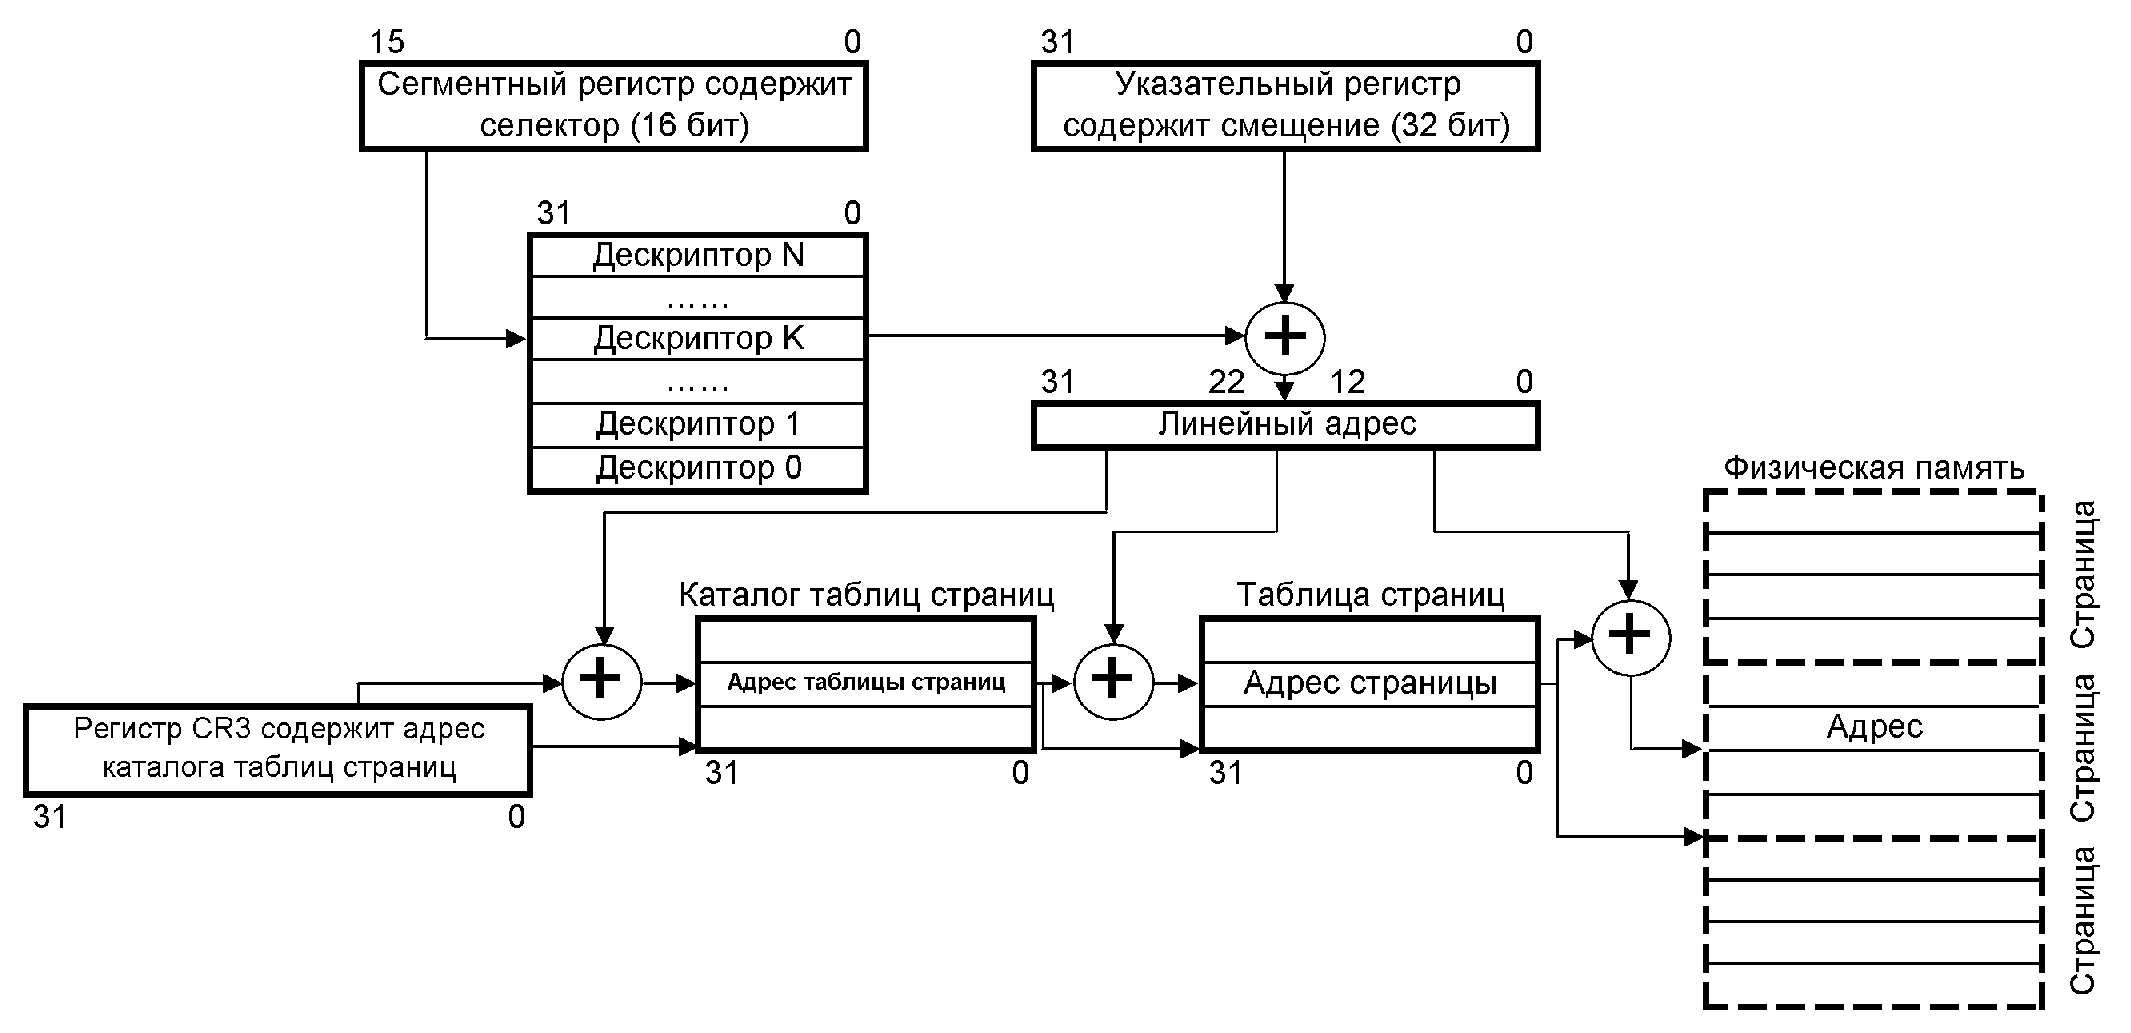
\includegraphics[height=0.8\textheight]{img/06.I8386_Addres_Translation.png}
        \caption{\href{https://en.wikipedia.org/wiki/Protected_mode}{Адресное преобразование 80386}}
    \end{figure}

    На иллюстрации опечатка, дескрипторы сегментов по 8 байт, а не по 4
\end{frame}

\begin{frame}{Расширения свыше 4 ГиБ}
    \begin{itemize}
        \item
        Устройства располагают свою память в 4-м ГиБ, так что, если
        установлено 4 ГиБ, часть памяти перекроется (будет недоступно).
        \item
        4 ГиБ может быть тоже мало.
    \end{itemize}

    Проблема решается при помощи Physical Address Extension --- доп.
    расширения, появившегося в Pentium Pro (на тот момент --- для серверов).
    Расширение позволяет страницам памяти располагаться не в контексте 4 ГиБ
    ОЗУ, а в контексте 64 ТиБ ОЗУ, по объему совпадающим с виртуальной
    памятью. При этом изменяется формат дескрипторов сегментов и страниц.

    Пользовательские процессы обычно не работают с памятью такого объема,
    для них всё выглядит по-старому. Картина меняется для ядра. Программы,
    которым объем памяти критичен, можно пересобрать со специальными
    библиотеками.
\end{frame}

\subsection{TODO: ARM и RISC-V}

\section*{}

\begin{frame}{Вопросы и упражнения}
    \small
    \vspace{-3mm}
    \begin{block}{Вопросы}
        \begin{itemize}
            \tightlist
            \item
            Программа выделила большой объём памяти, но не обращалась к ней.
            Сколько физической памяти было выделено?
            \item
            Опишите механизм сегментного преобразования
            \item
            Что такое адресное пространство, виртуальный и физический адреса?
            \item
            Что такое виртуальная память?
            \item
            Опишите механизм страничного преобразования
            \item
            Что такое замещение?
            \item
            Каким образом сегментная и страничная адресация позволяют изолировать
            программы в многозадачном режиме?
            \item
            Что такое Physical Address Extension?
        \end{itemize}
    \end{block}
    \vspace{-3mm}
    \begin{block}{Упражнения}
        \begin{itemize}
            \tightlist
            \item
            Напишите программу, выделяющую много (больше размера Вашего ОЗУ)
            памяти, но не обращающуюся к ней; понаблюдайте над расходом физической
            памяти
            \item
            Допишите программу выше, чтобы она интенсивно работала с памятью;
            опишите наблюдаемый эффект
            \item
            Повторите подобный эксперимент в меньших масштабах, измерьте, во
            сколько раз эффективная работа кэш-памяти ускоряет обращение к ОЗУ
        \end{itemize}
    \end{block}
\end{frame}

\postamble

\end{document}
